\section{Durchführung}
Im ersten Versuchsteil wird zunächst die Leerlaufspannung und der Innenwiderstand einer Monozelle gemessen, indem diese direkt an ein Voltmeter angeschlossen wird.
Die von dem Voltmeter angezeigte Spannung und Widerstand werden aufgeschrieben.

Jenach wird die in Abbildung \eqref{fig:aufbau1} zu sehende Messchaltung aufgebaut. Mit dieser wird die Klemmenspannung $U_{\text{k}}$ in Abhängigkeit vom Belastungsstrom $I$ gemessen.
Hierfür wird der regelbare Belastungswiderstand $R_{\text{a}}$ in einem Bereich von $0$ bis $50\,\symup{\Omega}$ variiert und 10 Messpaare $U_{\text{k}}$ und $I$ notiert.
   \begin{figure}[h!]
   \centering
   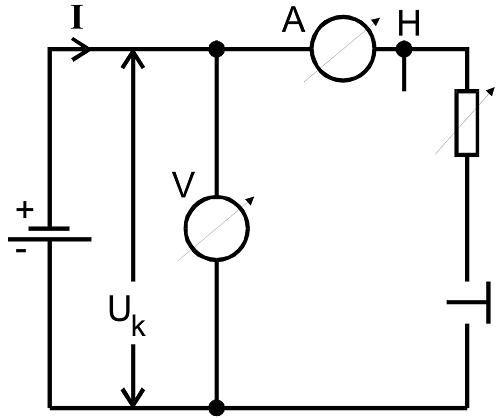
\includegraphics[width=0.4\linewidth]{aufbau1.png}
   \caption{Messschaltung zur Bestimmung von Leerlaufspannung und Innenwiderstand.}
   \label{fig:aufbau1}
   \end{figure}

Als Nächstes wird, wie in Abbildung \eqref{fig:aufbau1} zu sehen, zusätzlich zum vorherigen Aufbau eine Gegenspannung von etwa 2\,V in Reihe geschaltet. Nun fließt der Strom in entgegengesetzte Richtung und es können wieder bei 
verschiedenen Widerständen zwischen $0$ und $50\,\symup{\Omega}$ 10 Messpaare aufgenommen werden.
   \begin{figure}[h!]
   \centering
   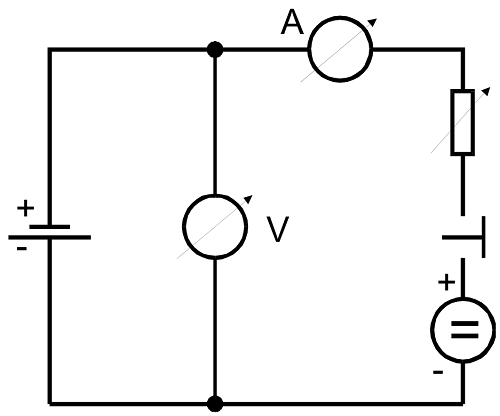
\includegraphics[width=0.4\linewidth]{aufbau2.png}
   \caption{Messschaltung mit Verwendung einer Gegenspannung.}
   \label{fig:aufbau2}
   \end{figure}

Zuletzt wird der zweite Versuchsteil wiederholt. Diesmal wird allerdings ein Generator statt der Monozelle und andere regelbare Widerstände verwendet. Bei der 1\,V-Rechteckspannung werden Widerstände im Bereich von 
$20$ bis $250\,\symup{\Omega}$ eingestellt, bei der 1\,V-Sinusspannung ist der Variationsbereich von $R_{\text{a}}$ $0{,}1$ bis $5\,\symup{k}\symup{\Omega}$. Für beide Spannungen werden jeweils 10 Wertepaare notiert.